%we don't want ae.sty
\expandafter\def\csname ver@ae.sty\endcsname{}

\documentclass[
  14pt,
  a1paper,
  portrait, 
  margin=0mm,
  innermargin=15mm,
  blockverticalspace=0mm,
  colspace=0mm,
  subcolspace=0mm
]{tikzposter}

\usepackage[T3]{fontenc}
\usepackage[utf8]{inputenc}
\usepackage[russian]{babel}

\usepackage{mhchem}
\usepackage{amssymb, amsmath}

\usepackage{tikz}
\usetikzlibrary{shapes.geometric, arrows, positioning, decorations.markings}
\usetikzlibrary{fit}
\usepackage{microtype}
\usepackage{framed}
\usetikzlibrary{decorations.pathmorphing,calc,backgrounds}

\usepackage{animate}

\usepackage{fixltx2e}
\usepackage{hyperref}

%\usetheme{Berkeley}
%\usetheme{Madrid} -- неплохо
%\usetheme{CambridgeUS}
%\usetheme{Singapore}
\usetheme{Warsaw}

\pdfmapfile{+sansmathaccent.map}

\title{Исследование бифуркаций в трехатомных гидридах методом классических траекторий}

\author{\small 
Финенко Артем \\[1ex] 
Научный руководитель: Петров С.В.}

\institute[MSU] % (optional, but mostly needed)
{
  МГУ им. М.В.Ломоносова \\
  Химический факультет
}

\date{23/12/2016}

\pgfdeclareimage[height=0.5cm]{university-logo}{../pictures/logo.jpg}
\logo{\pgfuseimage{university-logo}}

\newcommand\Fontvi{\fontsize{6}{7.2}\selectfont}

\beamertemplatenavigationsymbolsempty

\setbeamerfont{page number in head/foot}{size=\large}
\setbeamertemplate{footline}[frame number]
\setbeamertemplate{frametitle}[default][center]

% change font
\usefonttheme[onlymath]{serif}

% custom block environment
\newenvironment<>{varblock}[2][.9\textwidth]{%
  \setlength{\textwidth}{#1}
  \begin{actionenv}#3%
    \def\insertblocktitle{#2}%
    \par%
    \usebeamertemplate{block begin}}
  {\par%
    \usebeamertemplate{block end}%
  \end{actionenv}}

\tikzstyle{lagrange} = [rectangle, rounded corners, minimum width = 3cm, minimum height = 1cm, text centered, text width = 5cm, draw = black, fill=DarkOrchid!40]

\tikzstyle{equations} = [rectangle, rounded corners, text centered, draw = black, fill=green!30]

\tikzstyle{hamilton} = [rectangle, rounded corners, minimum width = 3cm, minimum height = 1cm, text centered, text width = 5 cm, draw = black, fill = Goldenrod!50]

\tikzstyle{result} = [rectangle, rounded corners, text centered, draw = black, fill = blue!30]

\tikzstyle{arrow} = [thick, ->, >=stealth]

\tikzstyle{vecArrow} = [thick, decoration={markings,mark=at position
   1 with {\arrow[semithick]{open triangle 60}}},
   double distance=1.4pt, shorten >= 5.5pt,
   preaction = {decorate},
   postaction = {draw,line width=1.4pt, white,shorten >= 4.5pt}]

\usepackage{caption}
\usepackage{subcaption}

\makeatletter
\def\TP@titlegraphictotitledistance{-9cm}
\settitle{ \centering \vbox{
    \@titlegraphic \\ [\TP@titlegraphictotitledistance] 
    \centering
    \color{titlefgcolor} {\bfseries \fontsize{1.5cm}{1cm}\selectfont \@title \par}
    \vspace*{1em}
    {\bfseries \fontsize{1.2cm}{1cm}\selectfont \@author \par} 
    \vspace*{1em} 
    {\bfseries \fontsize{1.2cm}{1cm}\selectfont \@institute}
}}
\makeatother

\newcommand{\SIZEOFTEXTREFERENCES}{\small}

\newcommand{\lb}{\left(}
\newcommand{\rb}{\right)}
\newcommand{\lsq}{\left[}
\newcommand{\rsq}{\right]}

\newcommand{\mL}{\mathcal{L}}
\newcommand{\mH}{\mathcal{H}}

\newcommand{\bbI}{\mathbb{I}}
\newcommand{\bOmega}{\boldsymbol{\Omega}}

\title{\parbox{0.75\linewidth}{\centering Использование методов статистической механики для расчета термодинамических и спектральных характеристик слабосвязанных молекулярных пар}}

\author{Чистиков Д., Финенко А.}
\institute{МГУ имени М.В. Ломоносова, Химический факультет}

\titlegraphic{
    
\includegraphics[width=6.5cm,height=5cm]{pictures/logo.jpg}
    \hfill 
    
\includegraphics[width=6.5cm,height=5cm]{pictures/logo.jpg}
    \vspace{5cm}
}

\usetheme{Simple}

\usepackage{amsmath,amssymb}

\newcommand{\vverh}{\vspace*{-0.1cm}}

\begin{document}
\maketitle[width=1.0\linewidth, titletotopverticalspace=0.1cm, titletoblockverticalspace=0.3cm]

\vspace*{-5cm}

\begin{columns}

\column{0.5}
\block[titleoffsety=1cm,bodyoffsety=2.5cm]{Введение}
{
	Интерес к теоретическому изучению слабосвязанных молекулярных пар в газах существует уже с серидины прошлого века, однако подобные исследования привлекают все больше внимания в связи с проблемами климатического моделирования в планетных атмосферах [1]. В последние годы было надежно установлено, что для построения достоверных климатических моделей планетных атмосфер необходим детальный учет эффектов слабого индуцированного поглощения в тепловой области спектра [1, 3]. Теория столкновительно-индуцированных спектров поглощения в газах, состоящих из молекул, не имеющих постоянного дипольного момента, на протяжении многих лет ограничивалась использованием сферически-симметричных потенциалов взаимодействия и модельных функций дипольного момента [2]. Расчет спектрального профиля является трудоемкой задачей, однако обратившись к методам статистической механики можно вычислить некоторые его характеристики, такие как спектральные моменты [2]. С использованием аналогичных методов могут быть получены другие характеристики [4], примерами которых служат второй вириальный коэффициент и константа равновесия образования ван-дер ваальсова комплекса. Все эти свойства оказываются полезными при моделировании спектров. Знание первых спектральных моментов позволяет сделать оценку спектрального профиля бинарного поглощения (см., например, [3]), а константа равновесия образования димеров позволяет оценить вклад димеров в интегральную интенсивность полос индуцированного поглощения (см., например, [5]). 
}

\block[titleoffsety=1.5cm,bodyoffsety=3cm]{Основные определения}
{
	В статистической термодинамике известно следующее выражение для константы равновесия реакции образования комплекса из двух мономеров
	\begin{gather}
			K_\textup{p}^\textup{bound} = \frac{Q_\text{bound}}{Q_{\text{mon}_1} Q_{\text{mon}_2}} \label{0.1},
	\end{gather}
	где через $Q_\text{bound}$ обозначена статистическая сумма димера, через $Q_{\text{mon}_1}$, $Q_{\text{mon}_2}$ -- статистические суммы мономеров. \par

	Коэффициент поглощения $\alpha(\nu)$ связан со спектральной функцией $g(\nu)$ следующим выражением [2] 
	\begin{gather}
		\frac{\alpha \lb \nu \rb}{\rho_1 \rho_2} = \frac{\lb 2 \pi \rb^3 N_L^2}{3 \hbar} \, \nu \left[ 1 - \exp \lb - \frac{h c \nu}{k T} \rb \right] g \lb \nu \rb, \label{0.2}
\end{gather}
где $N_L$ -- константа Лошмидта, $\hbar$ -- приведенная постоянная Планка, $k$ -- постоянная Больцмана, $\rho_1, \rho_2$ -- плотности газов (в амага), $c$ -- скорость света. Спектральным моментом $n$-го порядка называют интеграл следующего вида
\vspace*{-0.5cm}
\begin{gather}
	M_n = \int\limits_{-\infty}^{\infty} \nu^n g(\nu) d \nu. \label{0.3}
\end{gather}

В классическом приближении нулевой момент вычисляется как среднее значение квадрата дипольного момента $\boldsymbol{\mu}^2$ по фазовому пространству пары 
\begin{gather}
	M_0 = \displaystyle \frac{\int \boldsymbol{\mu}^2 \exp \lb -H \lb \mathbf{q}, \mathbf{p}, \mathbf{J} \rb / k T \rb d \mathbf{q} \, d \mathbf{p}}{\int \exp \lb - H \lb \mathbf{q}, \mathbf{p}, \mathbf{J} \rb / k T \rb d \mathbf{q} \, d \mathbf{p}} \label{0.4}. 
\end{gather}

}

\block[titleoffsety=1.5cm,bodyoffsety=3cm]{Общее рассмотрение задачи}
{
	Классическая сумма по состояниям связанного димера представляет собой следующий фазовый интеграл
	\begin{gather}
			Q_{\textup{bound}}(T) = \frac{1}{s_b h^{(l + 6)}} \int\limits_{H - E_{c.m.} < 0} \exp \left( -\frac{H}{kT} \right) dx^{\textup{c.m.}} \, dy^\textup{c.m.} \, dz^\textup{c.m.} \, dp_x^\textup{c.m.} \, dp_y^\textup{c.m.} \, dp_z^\textup{c.m.} \, dq_i \, dp_i, \label{1.1}
	\end{gather}
	где $s_b$ -- число симметрии молекулярной пары, $l$ -- количество независимых координат $q_i$ ($1 \leqslant i \leqslant l$); компоненты векторов координат и импульсов центра масс молекулярной пары обозначены $\mathbf{R} = \lb x^\textup{c.m.}, y^\textup{c.m.}, z^\textup{c.m.} \rb$, $\mathbf{P} = \lb p_x^\textup{c.m.}, p_y^\textup{c.m.}, p_z^\textup{c.m.} \rb$. Обозначим через $\mH$ гамильтониан, получающийся при отделении энергии центра масс $\mH = H - \mathbf{P}^2/2M$, где $M$ -- общая масса пары. Интегрирование по переменным центра масс дает трансляционную сумму по состояниям
	\begin{gather}
			Q_\textup{bound} = \frac{1}{s_b h^l} \lb \frac{2 \pi M k T}{h^2} \rb^{3/2} V \int\limits_{\mH < 0} \exp \lb - \frac{\mH}{kT} \rb dq_i \, dp_i, \label{1.2}
	\end{gather}
	где через $V$ обозначен объем, в котором заключена рассматриваемая молекулярная пара. \par
	Дальнейшее рассмотрение статистической суммы $\eqref{1.2}$ будем вести в специальной системе координат, которую будем называть <<трансляционной>>, а угловые координаты и сопряженные к ним импульсы будем отмечать верхним индексом ''t''. Будем рассматривать общий случай взаимодействия двух жестких мономеров, выпишем соответствующий этому случаю гамильтониан и проследим за выражениями для связанной статистической суммы. 
	
	\vspace*{-0.5cm}
	\subsection*{Транслированная система}
	Поместим начало системы отсчета в центр масс системы как целого; параметризуем ось, соединяющую центры масс мономеров, сферическими углами $\Theta$, $\Phi$; обозначим вектор, направленный из центра масс первого мономера в центр масс второго, через $\mathbf{R}$. Для описания ориентации каждого из мономеров транслируем систему отсчета в их центры масс, введем тройки углов Эйлера $\lb \varphi_1^t, \theta_1^t, \psi_1^t \rb$, $\lb \varphi_2^t, \theta_2^t, \psi_2^t \rb$. Кинетическая энергия в форме Лагранжа в определенной системе имеет следующий вид
	\begin{gather}
		T_\mL = \frac{\mu}{2} \lsq \dot{R}^2 + R^2 \dot{\Theta}^2 + R^2 \dot{\Phi}^2 \sin^2 \Theta \rsq + \frac{1}{2} \bOmega_1^\top \bbI_1 \bOmega_1 + \frac{1}{2} \bOmega_2^\top \bbI_2 \bOmega_2, \qquad \mu = \frac{m_{\textup{mon}_1} m_{\textup{mon}_2}}{m_{\textup{mon}_1} + m_{\textup{mon}_2}}, \label{1.3} 
	\end{gather}
	где через $m_{\textup{mon}_1}$ и $m_{\textup{mon}_2}$ обозначены массы мономеров, через $\mu$ -- приведенная масса молекулярной пары, через $\bbI_1 = \textup{diag} \lb I_\alpha^1, I_\beta^1, I_\gamma^1 \rb $, $\bbI_2 = \textup{diag} \lb I_\alpha^2, I_\beta^2, I_\gamma^2 \rb $ -- матрицы тензоров инерции мономеров в главных осях. Выражаем вектора угловой скорости $\bOmega_1, \bOmega_2$ через соответствующие вектора эйлеровых скоростей $\dot{\mathbf{e}}_1^t$, $\dot{\mathbf{e}}_2^t$; применяем стандартную процедуру перехода к гамильтоновой форме кинетической энергии, в ходе которой переходим от эйлеровых скоростей к эйлеровым импульсам $\mathbf{p}_1^t = \lb p_1^\varphi, p_1^\theta, p_1^\psi \rb$ и $\mathbf{p}_2^t = \lb p_2^\varphi, p_2^\theta, p_2^\psi \rb$.   
	\vspace*{-0.3cm}
	\begin{gather}
		T_\mH = \frac{p_R^2}{2\mu} + \frac{p_\Theta^2}{2 \mu R^2} + \frac{p_\Phi^2}{2 \mu R^2 \sin^2 \Theta} + \frac{1}{2 I_\alpha^2 \sin^2 \theta_2^t} \lsq \lb p_2^\varphi - p_2^\psi \cos \theta_2^t \rb \sin \psi_2^t + p_2^\theta \sin \theta_2^t \cos \psi_2^t \rsq^2 + \frac{1}{2 I_\beta^2 \sin^2 \theta_2^t} \times \notag \\
		\times \lsq \lb p_2^\varphi - p_2^\psi \cos \theta_2^t \rb \cos \psi_2^t  - p_2^\theta \sin \theta_2^t \sin \psi_2^t \rsq^2 + \frac{1}{2 I_\gamma^2} \lb p_2^\psi \rb^2 + \frac{1}{2 I_\alpha^1 \sin^2 \theta_1^t} \lsq \lb p_1^\varphi - p_1^\psi \cos \theta_1^t \rb \sin \psi_1^t + \right. \notag \\ 
		+ \left. p_1^\theta \sin \theta_1^t \cos \psi_1^t \rsq^2 + \frac{1}{2 I_\beta^1 \sin^2 \theta_1^t} \lsq \lb p_1^\varphi - p_1^\psi \cos \theta_1^t \rb \cos \psi_1^t - p_1^\theta \sin \theta_1^t \sin \psi_1^t \rsq^2 + \frac{1}{2 I_\gamma^1} \lb p_1^\psi \rb^2 \label{1.4}   
	\end{gather}

	Заметим, что потенциальная энергия в <<транслированной>> координатной системе будет зависеть от всех ввведенных координат $U = U \lb R, \Theta, \Phi, \varphi_1^t, \theta_1^t, \psi_1^t, \theta_2^t, \theta_2^t, \psi_2^t \rb$. Очертим последовательность преобразований, позволяющих перейти ко внутренним координатам $\left\{ R, \varphi_1, \varphi_2, \theta_1, \theta_2, \psi_1 \right\}$ внутри интегрального выражения \eqref{1.1}.
}
\column{0.5}
\block[titleoffsety=1cm,bodyoffsety=1.5cm]{}
{
	\vspace*{-2.0cm}
	\begin{tikzfigure}
	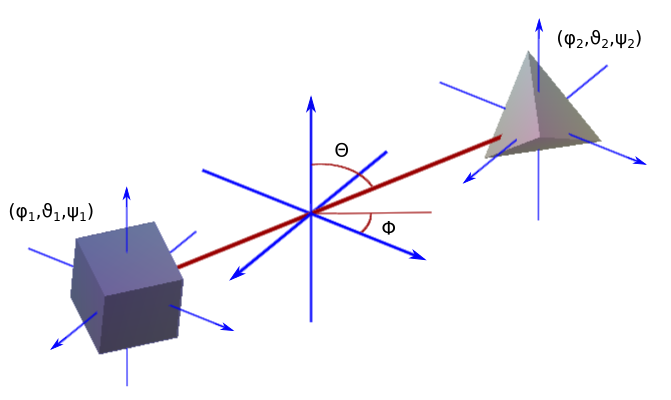
\includegraphics[scale=1.0]{./pictures/1.png}
\end{tikzfigure}
\begin{center}
		\vspace*{-1cm}
	Рис. 1. <<Транслированная>> система координат.	
\end{center}

	\vspace*{-0.5cm}
	\subsection*{Преобразование угловых переменных в интегральном выражении}
	Интегрирование в выражении $\eqref{1.2}$ ведется по области $\mH = T_\mH + U < 0$, где $T_\mH$ представлен формулой $\eqref{1.4}$. Осуществим тривиальную замену переменных, сводяющую кинетическую часть $\mH / kT$ к сумме квадратов
	\begin{gather}
		\frac{\mH}{kT} = x_1^2 + \dots + x_9^2 + \frac{U}{kT}, \quad \lsq \, \textup{Jac} \rsq = 2^{9 / 2} \mu^{3/2} R^2 \sqrt{I_\alpha^1 I_\beta^1 I_\gamma^1 I_\alpha^2 I_\beta^2 I_\gamma^2} \sin \Theta \sin \theta_1 \sin \theta_2. \label{1.5} 
	\end{gather}

	Представляя интеграл $\eqref{1.2}$ в виде повторного интеграла, в котором интегрирование во внешнем интеграле ведется по координатам, а интегрирование во внутренним интеграле -- по сопряженным им импульсам. Сделанная замена позволяет аналитически произвести интегрирование по импульсной части гамильтониана 
	\vspace*{-0.7cm}
	\begin{gather}
			Q_\textup{bound} = \frac{1}{s_b h^9} \lb \frac{2 \pi M k T}{h^2} \rb^{3/2} \int\limits_{U < 0} \frac{\displaystyle \gamma \lb \frac{9}{2}, - \frac{U}{k T} \rb}{\displaystyle \Gamma \lb \frac{9}{2} \rb} \lsq Jac \rsq dR \, d\Theta \, d\Phi \, d\varphi_1^t \, d\theta_1^t \, d\psi_1^t \, d\varphi_2^t \, d\theta_2^t \, d\psi_2^t, \label{1.5}
	\end{gather}
	где через $\gamma( \cdot, \cdot)$ и $\Gamma(\cdot)$ обозначены неполная и полная гамма-функции, соответственно. Используя формализм теории представлений группы вращений $SO(3)$ было показано, что внутри интеграла \eqref{1.5} можно перейти к переменным $\lb \varphi_1, \theta_1, \psi_1 \rb$, $\lb \varphi_2, \theta_2, \psi_2 \rb$, определяющим ориентацию мономеров относительно подвижной системы отсчета, причем само интегральное выражение остается неизменным. 

	Проводя алгебраические преобразования в формуле \eqref{1.5} приходим к следующему интегральному выражению для константы равновесия во внутренних переменных:
	\begin{gather}
			K_\textup{P}^\textup{bound} = \lb R T \rb^{-1} \frac{N_0}{8 \pi^2 s_b} \times \hspace{19cm} \notag \\
			\times \idotsint\limits_{U(R, \varphi_1, \theta_1, \psi_1, \varphi_2, \theta_2) < 0} \frac{\gamma \lb 9/2, - U / k T \rb}{\Gamma \lb 9 / 2 \rb} \exp \lb - \frac{U}{kT} \rb R^2 dR \, \sin \theta_1 d \theta_1 \sin \theta_2 d\theta_2 d \varphi_1 d \varphi_2 d \psi_1, \label{1.6}
	\end{gather}
	где через $Q_{\textup{mon}_1}$, $Q_{\textup{mon}_2}$ были обозначены статистические суммы мономеров, через $N_0$, $R$ -- число Авогадро и универсальная газовая постоянная, соответственно. Полученное выражение может быть легко упрощено для частных случаев взаимодействия мономеров с меньшим числом вращательных степеней свободы. 
}
\block[titleoffsety=1.5cm, bodyoffsety=2.5cm]{Температурные зависимости связанных статистических сумм и вклада димеров в нулевой спектральный момент}
{
	Полученные точные классические выражения могут быть использованы для усреднения величин, зависящих от внутренних координат, по фазовому пространству молекулярной пары. Использованный метод ползволяет выписать для таких средних значений интегральное выражение по области в конфигурационном пространстве, значительно упрощая вычислительную процедуру. Для иллюстрации вышесказанного приведем рассчитанные температурные зависимости констант равновесия и вклада димерных состояний в нулевой спектральный момент для разных систем.
	$\hspace*{-1.5cm}$
	\begin{minipage}{0.5\linewidth}
	\begin{tikzfigure}
	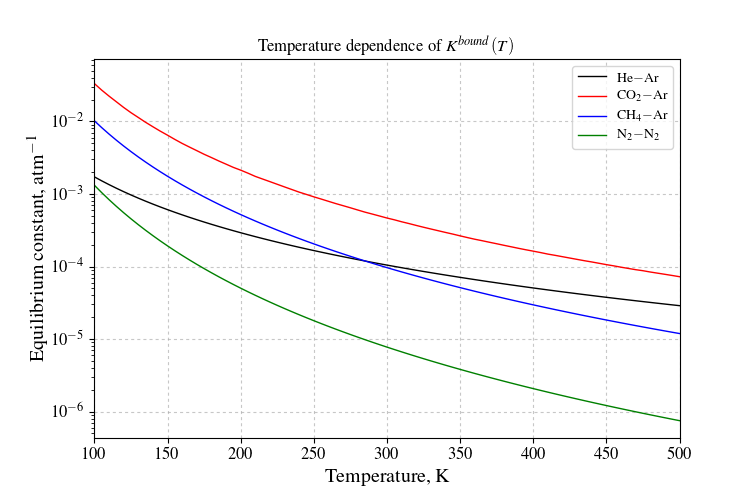
\includegraphics[scale=0.60]{./pictures/tdependencies.png}
	\end{tikzfigure}
	\end{minipage}
	$\quad \, \, \,$
	\begin{minipage}{0.5\linewidth}
	\begin{tikzfigure}
	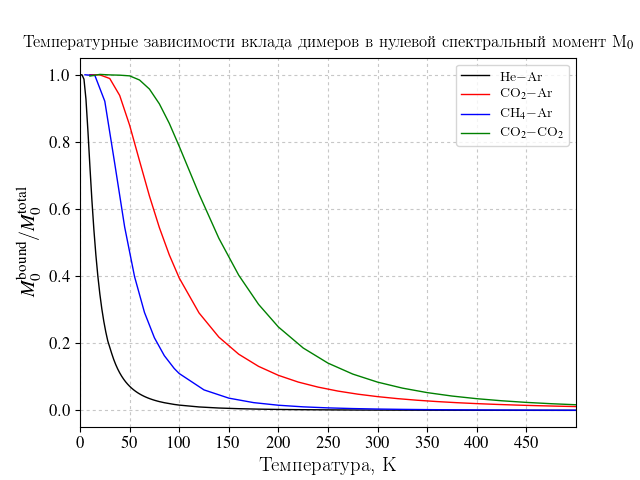
\includegraphics[scale=0.63]{./pictures/m0_bound_contribution.png}
	\end{tikzfigure}
	\end{minipage}
	\begin{center}
		Рис. 2-3. Температурные зависимости констант равновесия (слева) и вклада димеров в нулевой спектральный момент (справа).
	\end{center}
	
	\vspace*{-1.5cm}
	\begin{gather}
		\textup{He-Ar}: \quad K_\textup{P}^\textup{bound} = \frac{N_0}{R T} \int\limits_\sigma^{+\infty} \frac{\gamma \lb 3/2, -U(R) / kT \rb}{\Gamma \lb 3/2 \rb} \exp \lb -\frac{U}{kT} \rb R^2 dR, \quad U(\sigma) = 0 \notag \\
		\textup{CO$_2-$Ar}: \quad K_\textup{P}^\textup{bound} = \frac{2 \pi N_0}{R T} \iint\limits_{U(R, \theta) < 0} \frac{\gamma \lb 5/2, -U(R, \theta) / kT \rb}{\Gamma \lb 5/2 \rb} \exp \lb - \frac{U}{kT} \rb R^2 dR \, \sin \theta d\theta \notag \\ 
		\textup{CH$_4-$Ar}: \quad K_\textup{P}^\textup{bound} = \frac{N_0}{R T} \iiint\limits_{U(R, \theta, \phi) < 0} \frac{\gamma \lb 3, -U(R, \theta, \phi) / kT \rb}{\Gamma \lb 3 \rb} \exp \lb - \frac{U}{k T} \rb R^2 d R \, \sin \theta d\theta \, d\phi \notag \\
		\textup{N$_2-$N$_2$}: \quad K_\textup{P}^\textup{bound} = \frac{N_0}{4 R T} \idotsint\limits_{U(R, \theta_1, \theta_2, \phi) < 0} \frac{\gamma \lb 7/2, - U(R, \Omega)/kT \rb}{\Gamma \lb 7/2 \rb} \exp \lb -\frac{U}{kT} \rb R^2 dR \, \sin \theta_1 d\theta_1 \, \sin \theta_2 d\theta_2 \, d\phi \notag 
	\end{gather}
}
\block[titleoffsety=2.0cm, bodyoffsety=3.6cm]{Благодарности}
{
	Работа выполнена при частичной поддержке гранта РФФИ 18-05-00119. Авторы выражают благодарность С.Е. Локштанову, С.В. Петрову и А.А. Вигасину за неоценимую помощь.
}

\block[titleoffsety=1.5cm, bodyoffsety=3.2cm]{Список литературы}
{
\SIZEOFTEXTREFERENCES
%\hormove 1. \!\!C. Richard, I.\! E. Gordon, L.\! S. Rothman \textit{et al} (2012). New section of the HITRAN database: Collision-induced absorption (CIA). \textit{Journal of Quantitative Spectroscopy and Radiative Transfer}, 113(11), 1276-1285. \\ \hormove 
1. Vigasin, A.A., Mokhov, I.I. (2017). Izvestiya. Atmospheric and Oceanic Physics, 53, № 2, pp. 164-173. \\
2. Frommhold, L. (2006). Collision-induced absorption in gases. Cambridge University Press, 448pp. \\
3. Wordsworth, R., Kalugina, Y., Lokshtanov, S., Vigasin, A., Ehlmann, B., Head, J., Sanders, C. and Wang, H. (2017). Transient reducing greenhouse warming on early Mars, Geophysical Research Letters, 44(2), pp.665-671. \\
4. Hellmann, R., (2014). Chem. Phys. Lett., 613, pp.133-138. \\
5. Vigasin, A.A., (2000). Intensity and bandshapes of collision-induced absorption by CO2 in the region of the Fermi doublet. Journal of molecular spectroscopy, 200(1), pp.89-95.
}
\end{columns}

\end{document}
